\ylDisplay{Rong} % Ülesande nimi
{Tundmatu autor} % Autor
{piirkonnavoor} % Voor
{2016} % Aasta
{P 2} % Ülesande nr.
{1} % Raskustase
{
% Teema: Mehaanika
\ifStatement
Jaamast sõitu alustanud kaubarong kiirendas ühtlaselt ja saavutas $t_1=15$ minutiga kiiruse $v=80$ $km/h$. Sõitnud $t_2 = 2,5$ tundi ühtlase kiirusega, hakkas ta pidurdama ja ühtlaselt kiirust vähendades peatus $t_3=10$ minuti pärast järgmises jaamas. Kui suur oli rongi keskmine kiirus jaamadevahelisel teel?
\fi


\ifHint
Rongi poolt läbitud teepikkus on võrdne kiiruse graafiku aluse pindalaga.
\fi

\ifSolution
Keskmine kiirus avaldus järgmisest valemist.
\begin{center}
$v_k = \frac{s}{t} = \frac {s_1 + s_2 + s_3}{t_1 + t_2 + t_3}$
\end{center}
Liikumine koosneb kolmest etapist: kiirenev, ühtlane ja aeglustuv liikumine. Rongi poolt läbitud teepikkus on võrdne kiiruse graafiku aluse pindalaga.
\begin{center}
	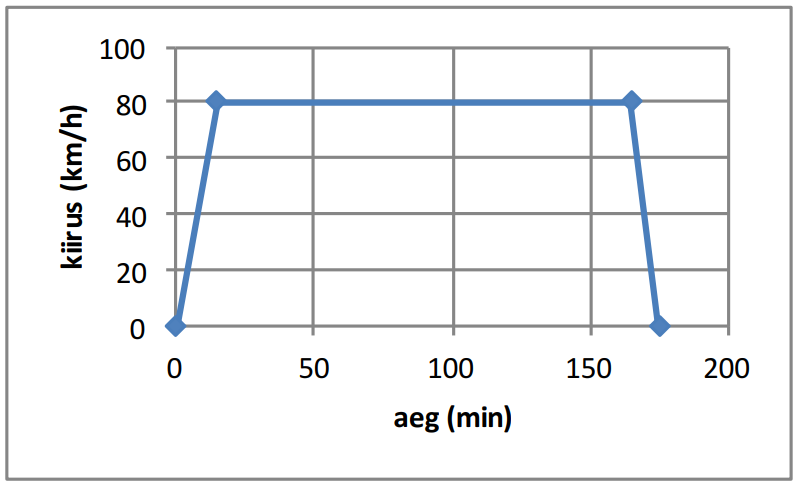
\includegraphics[width=0.5\linewidth]{2016-v2p-02-lah.png}
\end{center}
\begin{center}
$v_k = \frac{s}{t} = \frac{\cfrac{vt_1}{2} + vt_2 + \cfrac{vt_2}{2}}{t_1 + t_2 + t_3}$
\end{center}
Vastus $v_k = 74.3$ $km/h$
\fi
}